\documentclass[a4paper,12pt]{article}

\bibliographystyle{iopart-num}

\usepackage{graphicx}
\usepackage[hidelinks]{hyperref}
\usepackage[top=25mm,bottom=25mm,left=25mm,right=25mm]{geometry}
\usepackage{listings}
\usepackage{amsmath}
\usepackage{amssymb}
\usepackage{bm}
\usepackage[nocompress]{cite}
\usepackage[group-digits=integer]{siunitx}
\usepackage[font={it}]{caption}
\usepackage{placeins}
\usepackage{booktabs}
\usepackage{multicol}
\usepackage{float}
\graphicspath{ {images/} }

\title{Simulating Mixtures of Magnesium and Calcium Oxides}
\author{\textbf{Group 4}\\
	James Quirk\\
	Matthew Shelley\\
	George Watson}
\date{}


\begin{document}

\maketitle

\begin{abstract}
    
\end{abstract}

\begin{multicols}{2}
	
	Metal oxides such as magnesium and calcium oxide are of interest in solid state physics as they have a wide range of applications in thin film electronics such as flat-panel displays and flexible circuitry and sensors.\cite{kim2011lowtemperature} It is desirable to model the mixing of CaO and MgO to determine if it is feasible to fabricate components consisting of an alloy of MgO and CaO. In recent years, improvements in computational power have made it possible to model solid state structures computationally.
	\begin{center}
	    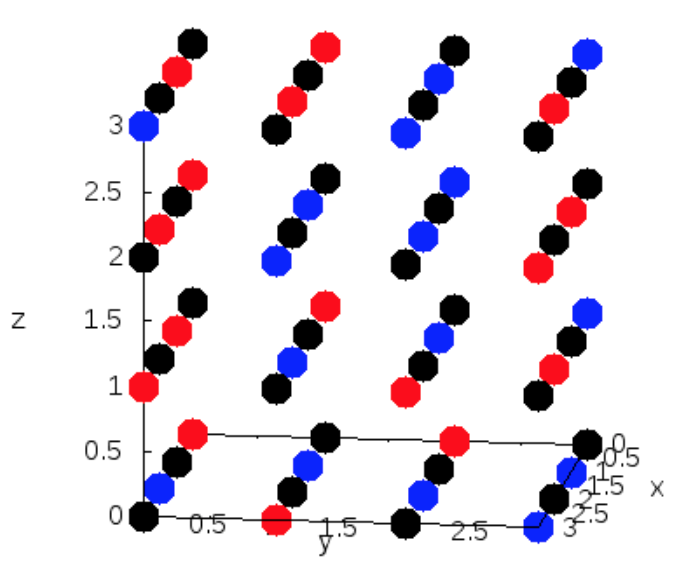
\includegraphics[keepaspectratio=true,width=0.4\textwidth]{lattice}
	    \captionof{figure}{Diagram demonstrating cubic lattice. Red is Mg, blue is Ca and black is O.}
			\label{fig:lattice} 
	\end{center}
	CASTEP\cite{clark2009first} was used to simulate simple cubic arrangement of magnesium, calcium, and oxygen. CASTEP uses density functional theory to model the structure; whilst very accurate, this process is extremely computationally expensive. A cube of randomly-arranged Mg and Ca in specified proportions (figure~\ref{fig:lattice}) actually represents an infinite crystal lattice due to the periodic boundary conditions used by CASTEP and allows the bulk properties of the substance to be considered. For computational efficiency, the positions of the atoms in the system were fixed and single-point optimisation was performed. This gives an upper bound for the energy of the system. In this simulation, a cube of 24 atoms was considered, allowing for testing of 14 different proportions of Mg and Ca. 
	
	The convex hull method\cite{jarvis1973identification} was used to draw conclusions about the lowest energy configurations. This involves drawing the convex shape with the smallest area around the data set, in this case only on the lower energy side since energy minimisation is the goal of the experiment. The method can be used to show that, for a given proportion of $\mathrm{Mg}/\mathrm{Ca}$ with an energy well inside the convex hull, it may be more energetically favourable for the material to be made from two separate sections with different proportions (but the same overall proportion), rather than a homogeneous mixture.
	
	Plotting the total energy (corrected for the finite basis set) against the proportion of calcium will produce a roughly linear set of data. This is because the individual energies associated with Mg and Ca are very different. Subtracting from this data the straight line formed by joining the first and last points should provide a better representation of the formation energy, which can then be used to plot a convex hull.
    \begin{center}
	    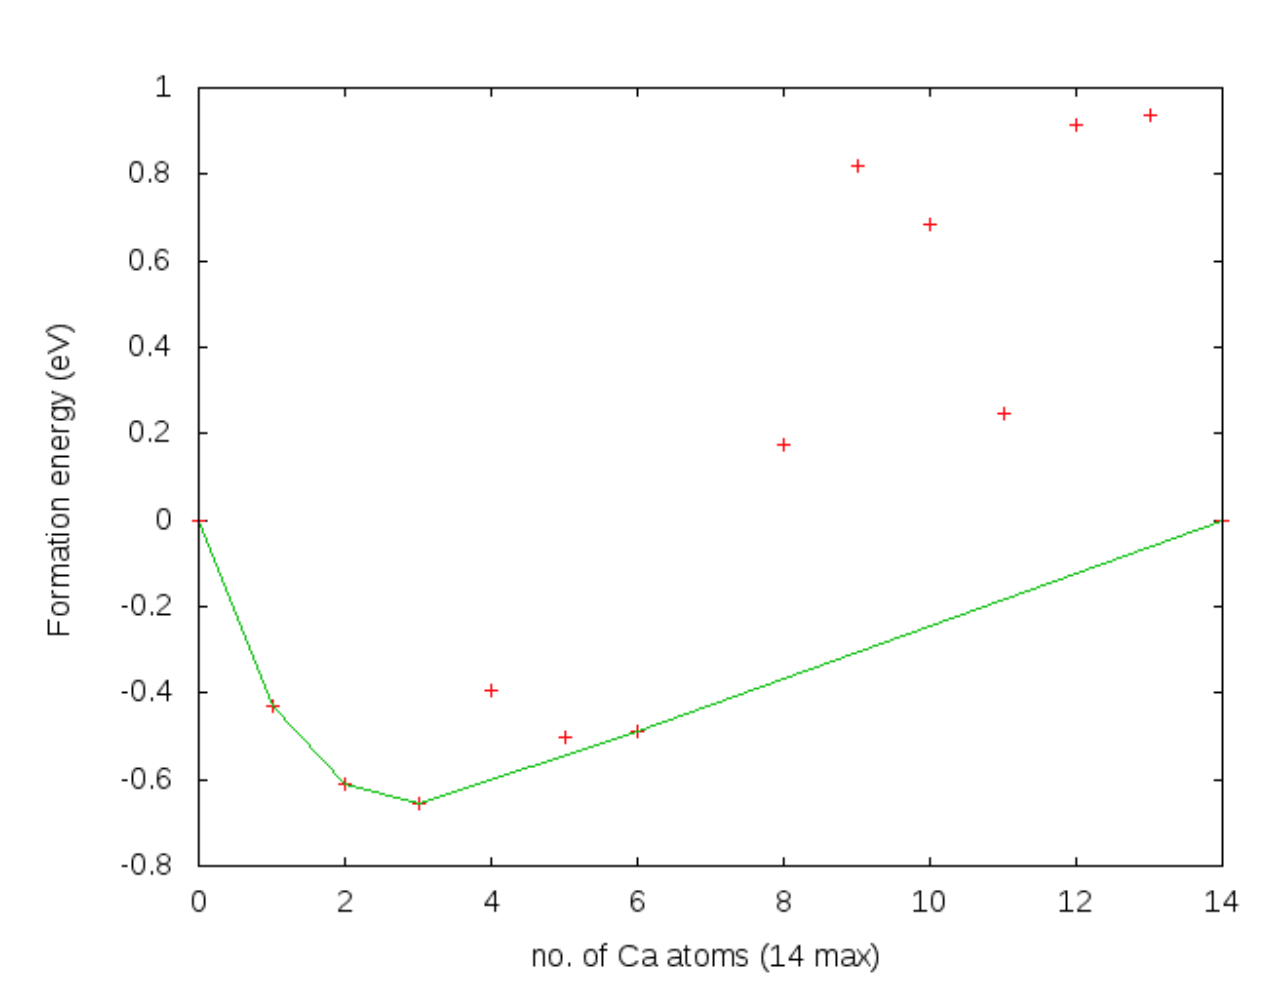
\includegraphics[keepaspectratio=true,width=0.4\textwidth]{convex}
	    \captionof{figure}{Convex hull diagram. The red points represent the formation energies determined from the deviation from the straight line fit. The green line is the convex hull.}
		\label{fig:convex} 
	\end{center}
    The results of the convex hull (Figure \ref{fig:convex}) were not as expected.  Clearly energies for a lattice of pure MgO or pure CaO had an energy of zero as these points exactly correspond with the straight line fit. When there was relatively little Ca in the lattice the results seemed well behaved but with higher concentrations of Ca formation energies rapidly became positive and the convex hull algorithm could not fit a well behaved parabola.
    
    This behaviour could be due to setting a fixed lattice and not optimising the geometry. Whilst the lattice set up for MgO may have been energetically favourable, Ca is a larger atom than Mg. With higher concentrations of Ca the fixed positions of the atoms may be packing them tighter than they would naturally form leading to the higher formation energies. These results could be improved by using the geometry optimisation feature of CASTEP. This will optimise the exact locations of particles in the lattice to find the most energetically favourable configuration. This is  an extremely computationally expensive process but would be possible with more time and reliable access to a supercomputer or cluster.
	
\raggedright
\bibliography{bibliography}

\end{multicols}
\end{document}